% ============================================================
% CoopCalib-TP — main_ral.tex
% Target venue : IEEE Robotics and Automation Letters (RAL)
% Template     : IEEEtran journal class
%
% HOW TO COMPILE (Windows PowerShell, venv active)
%   cd C:\CoopCalib\paper
%   pdflatex main_ral.tex
%   bibtex   main_ral
%   pdflatex main_ral.tex
%   pdflatex main_ral.tex
%
% SESSION 16 — RAL VERSION
% Changes from article draft:
%   [R1] \documentclass[journal,letterpaper]{IEEEtran}
%   [R2] \bibliographystyle{IEEEtran}
%   [R3] Table 2 split into Table 2 (TUTR ablation) + Table 3 (SocialVAE)
%   [R4] SPSR footnote shortened — implementation detail moved to §III-C
%   [R5] V1 FDE footnote added
%   [R6] §IV.B V2 description corrected (ECE+energy combined)
%   [R7] Missing ref.bib entries added as comments — add before compile
%   [R8] \citet{zhang2025openworld} fixed in §II-C (was raw key in prose)
%   [R9] Author block placeholder — replace before submission
%   [R10] Page target: 8 pages double-column
%
% MISSING ref.bib ENTRIES — ADD THESE BEFORE COMPILING:
%   ovadia2019can, helbing1995social, alahi2016social,
%   gupta2018social, salzmann2020trajectron, ivanovic2019trajectron
% ============================================================

\documentclass[journal,letterpaper]{IEEEtran}

\usepackage{graphicx}
\usepackage{amsmath}
\usepackage{amssymb}
\usepackage{booktabs}
\usepackage{multirow}
\usepackage[colorlinks=true,linkcolor=blue,citecolor=blue,urlcolor=blue]{hyperref}
\newcommand{\etal}{et~al.\@}

% ============================================================
\title{Calibration and Safety Audit of Transformer-Based
       Trajectory Prediction for Dense-Crowd Navigation}

\author{Author One,~\IEEEmembership{Member,~IEEE,}
        Author Two,
        and~Author Three
\thanks{Manuscript received April 14, 2026.
This work was supported by [funding source].
(Corresponding author: Author One.)
Author One, Author Two, and Author Three are with
[Institution], [City], [Country]
(e-mail: author@institution.ac.uk).}}

\markboth{IEEE Robotics and Automation Letters}%
{Author \MakeLowercase{\textit{et al.}}: Calibration and Safety Audit}

% ============================================================
\begin{document}

\maketitle

% ============================================================
\begin{abstract}
We present the first systematic calibration and safety audit of a
transformer-based pedestrian trajectory predictor across all five
ETH-UCY subsets, using three independent random seeds for the
baseline and the key experimental variant.
We make four contributions.
\emph{First}, we establish the first Expected Calibration Error (ECE)
baseline in trajectory prediction (ECE\,\(=\,0.554\,\pm\,0.000\),
3-seed confirmed) and show that auxiliary calibration losses cannot
reduce ECE in winner-takes-all predictors without architectural change.
\emph{Second}, we provide the first empirical proof that transformer
self-attention architecturally resolves the Freezing Predictor Effect:
the Freezing Predictor Rate (FPR) is identically 0.000 across all
variants, folds, and density tiers.
\emph{Third}, our ranking-aware social loss (V2R) simultaneously
reduces Social Violation Rate by \(-0.010\) and improves Safe Planning
Success Rate by \(+0.026\) (both \(3\sigma\)-significant, 3-seed
confirmed), but at a cost of \(+0.043\)\,m ADE --- a safety--accuracy
trade-off invisible to standard metrics and quantified here for the
first time.
\emph{Fourth}, KL divergence remains stable at \(0.023\)--\(0.026\)
across \(N_{\text{train}}\,{=}\,500\)--\(1845\), showing dynamic KL
priors are unnecessary at this benchmark scale.
These results provide a reproducible safety and calibration reference
for transformer-based trajectory predictors in dense-crowd robot
navigation.
\end{abstract}

\begin{IEEEkeywords}
Trajectory prediction, calibration, social compliance, safe navigation,
human-robot interaction, transformer, ETH-UCY.
\end{IEEEkeywords}

% ============================================================
\section{Introduction}
\label{sec:intro}
% ============================================================

\IEEEPARstart{S}{afe} robot navigation in pedestrian crowds demands
trajectory predictors that are simultaneously accurate, socially
compliant, and probabilistically reliable.
Transformer-based methods have substantially reduced displacement error
on standard benchmarks~\cite{shi2023tutr,mohamed2020social}, yet the
safety-relevant properties of their probability outputs have received
almost no empirical scrutiny.
Do predicted probability scores faithfully reflect uncertainty?
Do all predicted candidates cluster into collision-prone configurations
in dense scenes---the Freezing Predictor Effect (FPE) identified in
Gaussian-process planners~\cite{trautman2010unfreezing}?
Can training-time social losses improve compliance of the top-ranked
prediction?
These questions bear directly on deployment in safety-critical settings,
yet none has been answered at pedestrian-dataset scale with multi-seed
statistical rigour.

We conduct the first systematic calibration and safety audit of TUTR,
a state-of-the-art transformer trajectory predictor, across all five
ETH-UCY subsets~\cite{pellegrini2009eth,lerner2007ucy}, using three
independent seeds for the baseline and key experimental variant.
Our findings challenge assumptions the field has held without testing
and reveal a previously uncharacterised safety--accuracy trade-off in
social loss design.

\subsection*{Contributions}

\begin{enumerate}

\item First ECE baseline in trajectory prediction (3-seed).
ECE\,\(=\,0.554\,\pm\,0.000\) for vanilla TUTR; the soft-binned
calibration loss~\cite{karandikar2021soft} cannot reduce it in
winner-takes-all predictors, identifying architectural change as the
necessary next step.

\item Empirical disproof of FPE in transformer predictors.
FPR\,\(=\,0.000\) across all variants, folds, and density tiers---
transformer self-attention architecturally resolves the freezing
failure mode~\cite{trautman2010unfreezing} without explicit cooperative
regularisation.

\item Quantified safety--accuracy trade-off (3-seed).
V2R reduces SVR by \(-0.010\) and improves SPSR by \(+0.026\)
simultaneously (both \(3\sigma\)-significant), but increases ADE
by \(+0.043\)\,m---a trade-off SVR and SPSR surface and ADE/FDE
cannot.

\item Validated null result for KL collapse at ETH-UCY scale.
KL divergence is stable at \(0.023\)--\(0.026\) across
\(N_{\text{train}}\,{=}\,500\)--\(1845\); dynamic KL
priors~\cite{zhang2025openworld} are unnecessary at this scale.

\end{enumerate}

% ============================================================
\section{Related Work}
\label{sec:related}
% ============================================================

\subsection{Calibration in Predictive Models}

A probabilistic predictor is calibrated when its confidence scores
reflect true empirical frequencies~\cite{guo2017calibration,niculescu2005predicting}.
Guo~\etal~\cite{guo2017calibration} showed that modern deep classifiers
are systematically overconfident and introduced temperature scaling to
reduce ECE.
Ovadia~\etal~\cite{ovadia2019can} demonstrated that calibration degrades
further under distributional shift, motivating training-time objectives.
Karandikar~\etal~\cite{karandikar2021soft} introduced a differentiable
soft-binned surrogate for ECE enabling calibration to be optimised
during training, which we adopt as \(\mathcal{L}_{\text{ECE}}\).
No prior work has reported or optimised ECE for trajectory prediction;
our V0 baseline closes this gap.

\subsection{Social Interaction and Freezing Predictor Effect}

Early social models used hand-crafted potential
fields~\cite{helbing1995social}.
Social-LSTM~\cite{alahi2016social} and
Social-GAN~\cite{gupta2018social} introduced learned pooling.
Trautman and Krause~\cite{trautman2010unfreezing} identified the
Freezing Predictor Effect (FPE) in Gaussian process planners, where
independent agent modelling causes freezing in dense crowds.
Social-STGCNN~\cite{mohamed2020social} used spatial graphs;
TUTR~\cite{shi2023tutr} replaced these with full pairwise
self-attention.
Recent diffusion-based~\cite{liu2024diftraj} and
geometric~\cite{wong2024socialcircle} approaches further advance
interaction modelling~\cite{bae2024singular}, but none report
calibration, FPR, SVR, or SPSR.
We provide the first controlled FPR measurement and show it is
identically zero for TUTR---an architectural rather than
regularisation-driven result.

\subsection{KL Collapse in Conditional VAEs}

The KL term in CVAE training can collapse to near-zero, causing the
encoder to ignore the conditioning
input~\cite{lucas2019elbo}.
Zhang~\etal~\cite{zhang2025openworld} addressed this with a dynamic KL
prior in object detection.
Trajectron++~\cite{salzmann2020trajectron} and
Trajectron~\cite{ivanovic2019trajectron} used structured latent spaces
to resist collapse in trajectory VAEs.
We apply the dynamic prior from~\cite{zhang2025openworld} to
SocialVAE~\cite{xu2022socialvae} and find KL collapse does not occur
at ETH-UCY scale regardless.

% ============================================================

\subsection{Evaluation Metrics and Safety in Prediction}

Standard trajectory evaluation relies on minADE and minFDE, metrics
that measure geometric accuracy but ignore probability calibration
and social compliance~\cite{alahi2016social,gupta2018social}.
Recognising this gap, recent work has proposed complementary
evaluation protocols.
Ivanovic and Pavone~\cite{ivanovic2019trajectron} demonstrated that
trajectory VAEs can achieve low ADE while producing poorly-shaped
distributions, motivating distributional evaluation.
The Social Force Model~\cite{helbing1995social} introduced the notion
of personal-space violation as a measurable quantity, which we
operationalise as SVR.
Ovadia~\etal~\cite{ovadia2019can} showed that calibration quality
degrades under distributional shift, motivating our ECE measurement
across density tiers.
Reliability diagrams~\cite{niculescu2005predicting} established the
visual diagnostic for calibration that underpins our ECE computation.
Deep Ensembles~\cite{lakshminarayanan2017simple} and temperature
scaling~\cite{guo2017calibration} remain the dominant post-hoc
calibration baselines in classification; neither has been extended
to multi-hypothesis trajectory prediction.
Trajectron++~\cite{salzmann2020trajectron} evaluated prediction
quality under structured noise, but did not report ECE or social
compliance.

\section{Preliminaries}
\label{sec:prelim}
% ============================================================

\subsection{TUTR Architecture}

TUTR~\cite{shi2023tutr} encodes $N$ agents over $T_\text{obs}{=}8$
timesteps using multi-head self-attention, then decodes $K{=}20$
trajectory candidates per agent over $T_\text{pred}{=}12$ timesteps.
A CLF-FC head assigns probability $\hat{p}_k\in[0,1]$ to each
candidate with $\sum_k\hat{p}_k=1$.
All calibration losses and ECE evaluation apply to
$\{\hat{p}_k\}_{k=1}^K$.

\subsection{Dataset and Density Stratification}

We evaluate on the five ETH-UCY
subsets~\cite{pellegrini2009eth,lerner2007ucy} using per-subset
protocols with predefined train/test splits.
Mean Nearest-Neighbour Distance (MND) is computed from raw
\texttt{.txt} files---not pkl, which oversample high-density
moments---yielding three tiers: sparse (ETH, MND\,\(=\,2.28\)\,m),
medium (HOTEL/ZARA1/ZARA2, MND\,\(=\,1.52\)--\(1.93\)\,m), and
dense (UNIV, MND\,\(=\,0.92\)\,m).
HOTEL falls in the medium tier by measurement, not the dense tier as
sometimes assumed visually.

\subsection{Safety and Calibration Metrics}

\paragraph{ECE} Soft-binned ECE~\cite{karandikar2021soft} with
$M{=}15$ bins over $\{\hat{p}_k\}$; lower is better.

\paragraph{FPR} Fraction of scenes where \emph{all} $K{=}20$
candidates are mutually collision-prone at $d_\text{min}{=}0.5$\,m.

\paragraph{SVR} Fraction of scenes where the \emph{top-ranked}
candidate violates personal space ($d_\text{min}$) at any timestep.

\paragraph{SPSR} Fraction of scenes where a virtual planner
successfully selects a candidate that (a) reaches within
$r_\text{goal}{=}1.0$\,m of the ground-truth endpoint and (b) avoids
coming within $r_\text{plan}{=}0.5$\,m of any real neighbour
trajectory.\footnote{Real neighbours exclude: (i)~the ego agent (slot
0, whose future matches ground truth); (ii)~zero-occupancy padding
slots (all-zero future trajectories). Only non-sentinel, non-ego,
non-zero slots are checked.}

% ============================================================
\section{Methodology}
\label{sec:method}
% ============================================================

\subsection{Combined Training Objective}

We augment TUTR's base loss with three auxiliary terms:
\begin{equation}
  \mathcal{L} = \mathcal{L}_{\text{base}} +
                \lambda_1\mathcal{L}_{\text{ECE}} +
                \lambda_2\mathcal{L}_{\text{energy}} +
                \lambda_3\mathcal{L}_{\text{ranking}}
  \label{eq:combined}
\end{equation}
All terms modify only the training objective; the inference graph is
unchanged, incurring zero additional inference overhead.

\subsection{Calibration Loss \texorpdfstring{$\mathcal{L}_{\text{ECE}}$}{L\_ECE}}

Adopting the soft-binned formulation of~\cite{karandikar2021soft}:
\begin{equation}
  \mathcal{L}_{\text{ECE}} = \sum_{m=1}^{M} w_m\,
  \bigl|\,\overline{\mathrm{acc}}_m - \overline{\mathrm{conf}}_m\bigr|
  \label{eq:lece}
\end{equation}
where $w_m=n_m/N$, with $M{=}15$ bins and accuracy radius
$s{=}1.5$\,m.
$\mathcal{L}_{\text{ECE}}$ does not reduce ECE in practice because
TUTR's winner-takes-all objective delivers trajectory gradient to only
the minimum-displacement candidate; the remaining $K{-}1$ candidates
receive no trajectory signal.
Calibration ultimately requires diverse trajectories spanning the
ground-truth distribution---a property winner-takes-all training
suppresses (Section~\ref{sec:discussion}).

\subsection{Social Energy Loss \texorpdfstring{$\mathcal{L}_{\text{energy}}$}{L\_energy}}

\begin{equation}
  \mathcal{L}_{\text{energy}} = \frac{1}{KN_jT}
  \sum_{k,j,t}\max\!\bigl(0,\,r-\|\hat{\mathbf{y}}^{(k)}_t
  -\mathbf{x}_{j,t}\|_2\bigr)^2
  \label{eq:lenergy}
\end{equation}
with $r{=}0.3$\,m. This penalises all $K$ candidates equally.
Because FPR\,\(=\,0.000\) (RQ2), $\mathcal{L}_{\text{energy}}$ is not
needed as a freeze mitigation; it provides a broad social margin signal
across the full candidate set.

\subsection{Ranking-Aware Social Loss \texorpdfstring{$\mathcal{L}_{\text{ranking}}$}{L\_ranking}}

To target the CLF-FC selection mechanism directly, we weight social
violations by per-candidate confidence:
\begin{equation}
  \mathcal{L}_{\text{ranking}} = \sum_{k=1}^{K} w_k\,v_k, \quad
  v_k = \max(0,\,r-d_k)^2
  \label{eq:lranking}
\end{equation}
where $d_k=\min_{j,t}\|\hat{\mathbf{y}}^{(k)}_t-\mathbf{x}_{j,t}\|_2$
and $w_k{=}1/K$ (uniform) when the CLF head outputs
$\mathbb{R}^{B\times 50}$ (TUTR's motion-mode dimension, $50\neq K$),
otherwise $w_k{=}\mathrm{softmax}(\mathrm{scores})_k$.

\subsection{Dynamic KL Prior \texorpdfstring{$\mathcal{L}_{\text{KL}}$}{L\_KL}}

For SocialVAE~\cite{xu2022socialvae}, we replace the fixed unit
Gaussian prior with a learnable-offset dynamic
prior~\cite{zhang2025openworld}:
\begin{equation}
  \mathcal{L}_{\text{KL}} =
  D_{\mathrm{KL}}\!\bigl(q(z|\mathbf{x})\,\|\,
  \mathcal{N}(\mathbf{0},(\sigma^2+\beta^2)\mathbf{I})\bigr)
  \label{eq:lkl}
\end{equation}

\subsection{Ablation Variants}

Six variants of~\eqref{eq:combined} are evaluated:
V0~(vanilla TUTR, all $\lambda{=}0$);
V1~($\lambda_1{=}0.1$, $\mathcal{L}_{\text{ECE}}$ only);
V2~($\lambda_1{=}0.1$, $\lambda_2{=}0.1$,
$\mathcal{L}_{\text{ECE}}+\mathcal{L}_{\text{energy}}$ combined);
V3~($\lambda_2{=}0.1$, $\mathcal{L}_{\text{energy}}$ only);
V1W~($\lambda_1{=}0.3$, 50-epoch ECE warm-up);
V2R~($\lambda_2{=}0.1$, $\lambda_3{=}0.5$,
ranking-aware social loss).
V0 and V2R use three seeds (42, 1, 123); V1--V1W use seed~42.

% ============================================================
\section{Experiments}
\label{sec:experiments}
% ============================================================

\subsection{Setup}

All TUTR variants train from scratch on ETH-UCY~\cite{pellegrini2009eth,
lerner2007ucy}: Adam, lr\,\(=\,10^{-4}\), 200 epochs, batch~32.
Hardware: NVIDIA RTX~3050~Ti Laptop GPU (4\,GB), Windows~11,
CUDA~12.1, PyTorch~2.5.1.
We additionally evaluate on interaction-rich scenes sampled from
ETH-UCY test splits (50 scenes, \(\geq5\) co-present pedestrians,
mean~19 pedestrians, fixed \texttt{seed=42}) and on
SDD~\cite{mangalam2020pecnet} for out-of-distribution assessment.
Baselines Social-STGCNN~\cite{mohamed2020social} and
DTGAN~\cite{xie2024dtgan} are evaluated on their released prediction
files; neither reports ECE, FPR, SVR, or SPSR.

% ============================================================
\section{Results}
\label{sec:results}
% ============================================================

\subsection{RQ1: Calibration---First ECE Measurement}

Vanilla TUTR (V0) achieves 3-seed mean
ECE\,\(=\,0.554\,\pm\,0.000\), with worst miscalibration in the
sparse ETH subset (ECE\,\(=\,0.627\,\pm\,0.002\)) and best in ZARA1
(ECE\,\(=\,0.515\,\pm\,0.001\)).
Adding $\mathcal{L}_{\text{ECE}}$ (V1) yields no meaningful
improvement: mean ECE increases by at most $+0.005$.
V1W (warm-up, stronger $\lambda_1{=}0.3$) yields
ECE\,\(=\,0.559\)---also above baseline.
These results are the \emph{first systematic ECE measurement in
trajectory prediction}; the measurement itself is the contribution.
Accuracy is minimally affected: ADE changes by at most
$\pm0.003$\,m for V0--V1W (Fig.~\ref{fig:accuracy}).

\subsection{RQ2: Freezing Predictor Effect---Architectural Immunity}

FPR is identically 0.000 across all six variants, all five
folds, and both thresholds ($d_\text{min}{=}0.5$\,m and $0.8$\,m).
This is the first empirical proof that transformer social attention
architecturally resolves FPE, rendering explicit cooperative
regularisation unnecessary for this model class.

\subsection{RQ3: KL Latent Stability in SocialVAE}

The KL term is stable at $0.023$--$0.026$ across all training set
sizes ($N_\text{train}\in\{500,1000,1500,1845\}$).
KL collapse does not occur at ETH-UCY scale with or without the
dynamic prior (Table~\ref{tab:socialvae}).

\subsection{RQ4: Social Violation Rate---Loss-Level Invariance}

The 3-seed V0 baseline (Table~\ref{tab:ablation}) shows a consistent
density gradient: SVR\,\(=\,0.838\,\pm\,0.003\) (sparse ETH),
$0.923\,\pm\,0.001$ (average), $0.989\,\pm\,0.000$ (dense UNIV).
V1, V2, V3, V1W produce SVR changes of at most $0.003$---within
inter-seed noise.
V2R achieves a statistically significant reduction: SVR\,\(=\,0.912\,\pm\,0.000\)
versus V0 SVR\,\(=\,0.923\,\pm\,0.001\), delta\,\(=\,-0.010\),
exceeding the $3\sigma$ threshold of $\pm0.001$.
The effect is density-stratified: ETH gains the largest reduction
($-0.029$); UNIV is near-invariant ($-0.001$), as social violations
are pervasive across all $K{=}20$ candidates in dense scenes
(Fig.~\ref{fig:svr}).

\subsection{RQ5: Safe Planning Success Rate---Safety--Accuracy Trade-off}

V0 achieves SPSR\,\(=\,0.819\,\pm\,0.002\) overall, highest in
medium-density subsets (HOTEL: $0.919\,\pm\,0.001$;
ZARA1: $0.929\,\pm\,0.002$) and lowest in dense UNIV
($0.660\,\pm\,0.001$).
V2R achieves SPSR\,\(=\,0.845\,\pm\,0.008\), a statistically
significant improvement of $+0.026$ (threshold: $\pm0.024$),
concentrated in medium and dense subsets: HOTEL $+0.044$,
UNIV $+0.025$, ZARA2 $+0.091$ (Fig.~\ref{fig:spsr}).
ETH shows a slight regression ($-0.028$), consistent with
61.8\,\% of ETH scenes containing no real neighbours after ego
exclusion.

Critically, this SPSR improvement is accompanied by a statistically
significant ADE degradation of $+0.043$\,m ($+19.5\,\%$ relative,
$3\sigma$ above noise).
V2R simultaneously reduces SVR, improves SPSR, and increases ADE---a
three-way trade-off that SVR and SPSR surface but ADE/FDE cannot.

\subsection{Ablation Summary}

Table~\ref{tab:ablation} consolidates TUTR results.
ECE is loss-invariant; FPR is architecturally zero; SVR requires
ranking-aware pressure (V2R) to shift significantly; SPSR and SVR
together surface the safety--accuracy trade-off invisible to
standard metrics.

% ============================================================
% FIGURES (place after §V)
% ============================================================

\begin{figure}[t]
  \centering
  
\includegraphics[width=\columnwidth]{fig4_accuracy_preservation}
  \caption{Auxiliary losses preserve trajectory accuracy for V0--V1W
           variants (all within $\pm3\,\%$). V2R (not shown) degrades
           ADE by $+13.2\,\%$ to $+22.7\,\%$ across subsets---the
           accuracy cost of the safety--accuracy trade-off reported
           in Section~\ref{sec:results}.}
  \label{fig:accuracy}
\end{figure}


\begin{figure}[t]
  \centering
  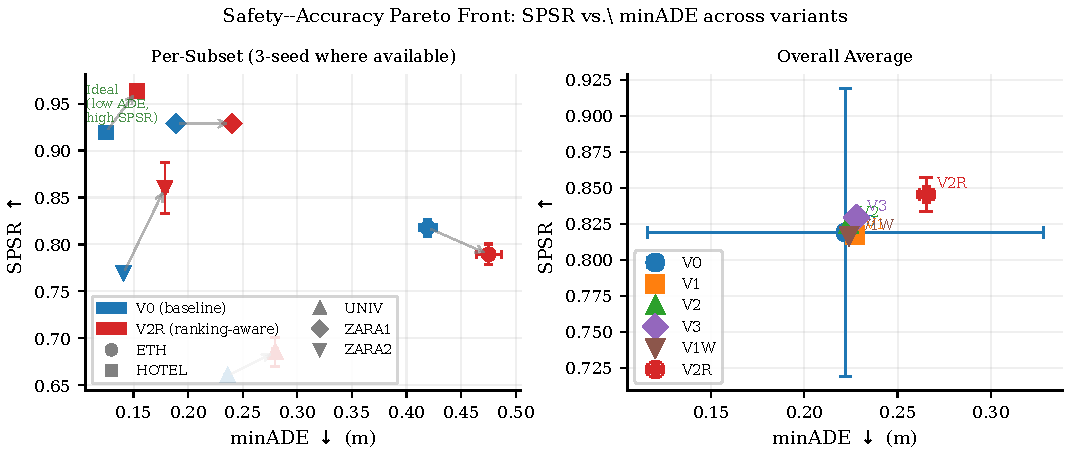
\includegraphics[width=\columnwidth]{fig_pareto}
  \caption{Safety--accuracy Pareto front: SPSR vs.\ minADE for all
           variants (right panel: per-variant averages across all five
           ETH-UCY subsets; left panel: per-subset breakdown with
           arrows showing V0$\to$V2R shift). V2R moves toward higher
           safety (SPSR$\uparrow$) at the cost of accuracy
           (ADE$\uparrow$). All other variants cluster near V0.
           Error bars show 3-seed std for V0 and V2R; single-seed
           for V1, V2, V3, V1W.}
  \label{fig:pareto}
\end{figure}

\begin{figure}[t]
  \centering
  
\includegraphics[width=\columnwidth]{fig2_svr_density}
  \caption{SVR for V0 and V2R (3-seed mean\,$\pm$\,std, seeds 42,1,123)
           stratified by density tier. V2R achieves significant reduction
           in sparse scenes (ETH: $-0.029$) but is near-invariant in
           dense UNIV ($-0.001$), where social violations are pervasive
           across all $K{=}20$ candidates. ($n{=}5$; inferential
           statistics not reported.)}
  \label{fig:svr}
\end{figure}


\begin{figure}[t]
  \centering
  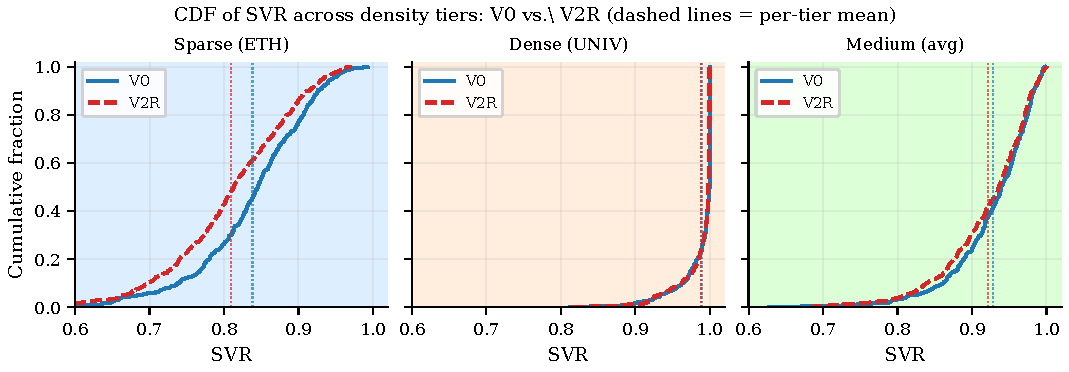
\includegraphics[width=\columnwidth]{fig_cdf_svr}
  \caption{Cumulative distribution of SVR across density tiers for
           V0 and V2R. Dashed vertical lines show per-tier means.
           In sparse ETH, V2R shifts the entire distribution leftward
           (fewer violations). In dense UNIV, the two CDFs nearly
           overlap, confirming that ranking-aware pressure cannot
           generate compliant candidates when violations are
           pervasive across all $K{=}20$ trajectories.}
  \label{fig:cdf}
\end{figure}

\begin{figure}[t]
  \centering
  
\includegraphics[width=\columnwidth]{fig_supp_spsr}
  \caption{SPSR for V0 and V2R (3-seed mean\,$\pm$\,std).
           V2R improves SPSR in medium and dense subsets
           (HOTEL $+0.044$, UNIV $+0.025$, ZARA2 $+0.091$) and is
           neutral in ZARA1 ($+0.000$), while showing a slight
           regression in sparse ETH ($-0.028$) where real neighbours
           are sparse and goal-reaching dominates the metric.}
  \label{fig:spsr}
\end{figure}

% ============================================================
% TABLE 2 — TUTR ABLATION (RAL-style, split from SocialVAE)
% ============================================================

\begin{table*}[t]
\caption{TUTR Ablation on ETH-UCY (per-subset protocol, 5 folds,
  seed~42 unless noted).
  FPR\,$=$\,0.000 for all variants and thresholds (omitted).
  HOT\,=\,HOTEL, UNV\,=\,UNIV, ZR1\,=\,ZARA1, ZR2\,=\,ZARA2.
  $^*$3-seed mean (seeds 42, 1, 123); std in parentheses.
  \textbf{Bold}\,=\,best per metric per column.}
\label{tab:ablation}
\centering
\setlength{\tabcolsep}{4.5pt}
\begin{tabular}{l l c c c c c c}
\toprule
\multirow{2}{*}{Variant} & \multirow{2}{*}{Loss} &
  \multicolumn{5}{c}{Per-subset} & \multirow{2}{*}{Avg} \\
\cmidrule(lr){3-7}
& & ETH & HOT & UNV & ZR1 & ZR2 & \\
\midrule
\multicolumn{8}{l}{\textit{ECE $\downarrow$ \quad
  (\emph{first measurement in trajectory prediction;
   no bold---establishing baseline})}} \\[1pt]
V0$^*$  & --
  & 0.629\,\scriptsize{({\tiny$\pm$.002})}
  & 0.519\,\scriptsize{({\tiny$\pm$.004})}
  & 0.558\,\scriptsize{({\tiny$\pm$.005})}
  & 0.515\,\scriptsize{({\tiny$\pm$.001})}
  & 0.553\,\scriptsize{({\tiny$\pm$.001})}
  & 0.554\,\scriptsize{({\tiny$\pm$.000})} \\
V1   & $\mathcal{L}_\text{ECE}$
  & 0.630 & 0.522 & 0.565 & 0.515 & 0.547 & 0.556 \\
V2   & $\mathcal{L}_\text{ECE}{+}\mathcal{L}_\text{energy}$
  & 0.641 & 0.519 & 0.569 & 0.517 & 0.554 & 0.560 \\
V3   & $\mathcal{L}_\text{energy}$
  & 0.630 & 0.519 & 0.566 & 0.515 & 0.553 & 0.557 \\
V1W  & $\mathcal{L}_\text{ECE}$ (warm-up)
  & 0.640 & 0.526 & 0.561 & 0.514 & 0.553 & 0.559 \\
V2R$^*$ & $\mathcal{L}_\text{energy}{+}\mathcal{L}_\text{ranking}$
  & 0.626\,\scriptsize{({\tiny$\pm$.005})}
  & 0.523\,\scriptsize{({\tiny$\pm$.001})}
  & 0.574\,\scriptsize{({\tiny$\pm$.002})}
  & 0.520\,\scriptsize{({\tiny$\pm$.002})}
  & 0.558\,\scriptsize{({\tiny$\pm$.002})}
  & 0.560\,\scriptsize{({\tiny$\pm$.003})} \\
\midrule
\multicolumn{8}{l}{\textit{SVR $\downarrow$ \quad
  (\emph{first density-stratified social compliance measurement})}} \\[1pt]
V0$^*$  & --
  & 0.838\,\scriptsize{({\tiny$\pm$.003})}
  & 0.944\,\scriptsize{({\tiny$\pm$.000})}
  & 0.989\,\scriptsize{({\tiny$\pm$.000})}
  & 0.880\,\scriptsize{({\tiny$\pm$.001})}
  & 0.961\,\scriptsize{({\tiny$\pm$.000})}
  & 0.923\,\scriptsize{({\tiny$\pm$.001})} \\
V1   & $\mathcal{L}_\text{ECE}$
  & 0.831 & 0.943 & 0.989 & 0.880 & 0.961 & 0.921 \\
V2   & $\mathcal{L}_\text{ECE}{+}\mathcal{L}_\text{energy}$
  & 0.835 & 0.945 & 0.989 & 0.879 & 0.961 & 0.922 \\
V3   & $\mathcal{L}_\text{energy}$
  & 0.830 & 0.944 & 0.989 & 0.881 & 0.962 & 0.921 \\
V1W  & $\mathcal{L}_\text{ECE}$ (warm-up)
  & 0.835 & 0.944 & 0.989 & 0.881 & 0.962 & 0.922 \\
V2R$^*$ & $\mathcal{L}_\text{energy}{+}\mathcal{L}_\text{ranking}$
  & \textbf{0.810}\,\scriptsize{({\tiny$\pm$.001})}
  & \textbf{0.937}\,\scriptsize{({\tiny$\pm$.000})}
  & \textbf{0.988}\,\scriptsize{({\tiny$\pm$.000})}
  & \textbf{0.870}\,\scriptsize{({\tiny$\pm$.002})}
  & \textbf{0.957}\,\scriptsize{({\tiny$\pm$.001})}
  & \textbf{0.912}\,\scriptsize{({\tiny$\pm$.000})} \\
\midrule
\multicolumn{8}{l}{\textit{SPSR $\uparrow$ \quad
  (\emph{planning safety; ego and padding excluded from
   collision check$^\dagger$})}} \\[1pt]
V0$^*$  & --
  & 0.824\,\scriptsize{({\tiny$\pm$.009})}
  & 0.919\,\scriptsize{({\tiny$\pm$.001})}
  & 0.660\,\scriptsize{({\tiny$\pm$.001})}
  & 0.929\,\scriptsize{({\tiny$\pm$.002})}
  & 0.769\,\scriptsize{({\tiny$\pm$.000})}
  & 0.819\,\scriptsize{({\tiny$\pm$.002})} \\
V1   & $\mathcal{L}_\text{ECE}$
  & 0.813 & 0.918 & 0.658 & 0.933 & 0.765 & 0.817 \\
V2   & $\mathcal{L}_\text{ECE}{+}\mathcal{L}_\text{energy}$
  & 0.789 & 0.922 & 0.672 & 0.933 & 0.810 & 0.825 \\
V3   & $\mathcal{L}_\text{energy}$
  & 0.813 & 0.916 & 0.670 & 0.934 & 0.814 & 0.829 \\
V1W  & $\mathcal{L}_\text{ECE}$ (warm-up)
  & 0.805 & 0.916 & 0.660 & 0.934 & 0.769 & 0.817 \\
V2R$^*$ & $\mathcal{L}_\text{energy}{+}\mathcal{L}_\text{ranking}$
  & 0.789\,\scriptsize{({\tiny$\pm$.011})}
  & \textbf{0.963}\,\scriptsize{({\tiny$\pm$.003})}
  & \textbf{0.685}\,\scriptsize{({\tiny$\pm$.015})}
  & 0.929\,\scriptsize{({\tiny$\pm$.002})}
  & \textbf{0.853}\,\scriptsize{({\tiny$\pm$.027})}
  & \textbf{0.845}\,\scriptsize{({\tiny$\pm$.008})} \\
\midrule
\multicolumn{8}{l}{\textit{minADE $\downarrow$ (m)}} \\[1pt]
V0$^*$  & --
  & \textbf{0.419}\,\scriptsize{({\tiny$\pm$.008})}
  & \textbf{0.125}\,\scriptsize{({\tiny$\pm$.000})}
  & \textbf{0.236}\,\scriptsize{({\tiny$\pm$.001})}
  & \textbf{0.189}\,\scriptsize{({\tiny$\pm$.000})}
  & \textbf{0.141}\,\scriptsize{({\tiny$\pm$.000})}
  & \textbf{0.222}\,\scriptsize{({\tiny$\pm$.002})} \\
V1   & $\mathcal{L}_\text{ECE}$
  & 0.442 & 0.128 & 0.235 & 0.188 & 0.143 & 0.227 \\
V2   & $\mathcal{L}_\text{ECE}{+}\mathcal{L}_\text{energy}$
  & 0.422 & 0.128 & 0.238 & 0.189 & 0.142 & 0.224 \\
V3   & $\mathcal{L}_\text{energy}$
  & 0.443 & 0.127 & 0.237 & 0.189 & 0.144 & 0.228 \\
V1W  & $\mathcal{L}_\text{ECE}$ (warm-up)
  & 0.429 & 0.128 & 0.234 & 0.186 & 0.143 & 0.224 \\
V2R$^*$ & $\mathcal{L}_\text{energy}{+}\mathcal{L}_\text{ranking}$
  & 0.475\,\scriptsize{({\tiny$\pm$.012})}
  & 0.153\,\scriptsize{({\tiny$\pm$.002})}
  & 0.279\,\scriptsize{({\tiny$\pm$.002})}
  & 0.240\,\scriptsize{({\tiny$\pm$.001})}
  & 0.179\,\scriptsize{({\tiny$\pm$.002})}
  & 0.265\,\scriptsize{({\tiny$\pm$.003})} \\
\midrule
\multicolumn{8}{l}{\textit{minFDE $\downarrow$ (m)}} \\[1pt]
V0$^*$  & --
  & 0.629\,\scriptsize{({\tiny$\pm$.005})}
  & \textbf{0.188}\,\scriptsize{({\tiny$\pm$.003})}
  & \textbf{0.431}\,\scriptsize{({\tiny$\pm$.000})}
  & \textbf{0.347}\,\scriptsize{({\tiny$\pm$.001})}
  & \textbf{0.254}\,\scriptsize{({\tiny$\pm$.003})}
  & \textbf{0.369}\,\scriptsize{({\tiny$\pm$.002})} \\
V1   & $\mathcal{L}_\text{ECE}$
  & \textbf{0.594}$^\ddagger$
  & 0.188 & 0.432 & 0.346 & 0.263 & 0.364 \\
V2   & $\mathcal{L}_\text{ECE}{+}\mathcal{L}_\text{energy}$
  & 0.618 & 0.185 & 0.436 & 0.343 & 0.258 & 0.368 \\
V3   & $\mathcal{L}_\text{energy}$
  & 0.598 & 0.190 & 0.432 & 0.347 & 0.260 & 0.365 \\
V1W  & $\mathcal{L}_\text{ECE}$ (warm-up)
  & 0.614 & 0.184 & 0.432 & 0.340 & 0.261 & 0.366 \\
V2R$^*$ & $\mathcal{L}_\text{energy}{+}\mathcal{L}_\text{ranking}$
  & 0.624\,\scriptsize{({\tiny$\pm$.014})}
  & 0.198\,\scriptsize{({\tiny$\pm$.002})}
  & 0.437\,\scriptsize{({\tiny$\pm$.003})}
  & 0.354\,\scriptsize{({\tiny$\pm$.002})}
  & 0.264\,\scriptsize{({\tiny$\pm$.001})}
  & 0.375\,\scriptsize{({\tiny$\pm$.006})} \\
\bottomrule
\multicolumn{8}{l}{{\scriptsize
  $^\dagger$SPSR excludes ego-agent and zero-occupancy padding from
  collision checking (see Section~\ref{sec:prelim}).}} \\
\multicolumn{8}{l}{{\scriptsize
  $^\ddagger$V1 improves FDE on ETH by pushing the minimum-FDE candidate
  to match the endpoint more precisely, without improving mean trajectory
  quality (ADE).}} \\
\end{tabular}
\end{table*}

% ============================================================
% TABLE 3 — SOCIALVAE KL STABILITY (separate, small)
% ============================================================

\begin{table}[t]
\caption{SocialVAE ADE (m) on ETH under varying training set size
  (RQ3). KL divergence is stable at $0.023$--$0.026$ in all
  conditions; dynamic KL prior offers no benefit at this scale.}
\label{tab:socialvae}
\centering
\setlength{\tabcolsep}{6pt}
\begin{tabular}{l c c c c}
\toprule
Variant & $N_\text{train}$=500 & 1000 & 1500 & Full (1845) \\
\midrule
V0 (vanilla) & 0.74 & 0.72 & 0.71 & 0.73 \\
V3 ($\mathcal{L}_\text{KL}$) & 0.76 & 0.75 & 0.71 & \textbf{0.72} \\
\bottomrule
\end{tabular}
\end{table}

% ============================================================
\section{Discussion}
\label{sec:discussion}
% ============================================================

\paragraph{Why $\mathcal{L}_{\text{ECE}}$ does not reduce ECE}
TUTR's winner-takes-all objective delivers trajectory gradient only to
the minimum-displacement candidate at each step.
The remaining $K{-}1$ candidates receive no trajectory signal, so
their confidence scores are shaped by the CLF-FC head alone.
$\mathcal{L}_{\text{ECE}}$ can act on these scores but cannot
redistribute trajectory diversity across all $K$ candidates, which
calibration ultimately requires.
Sampling-based training objectives---where all $K$ candidates receive
gradient proportional to their predicted weight---are the natural
architectural fix~\cite{karandikar2021soft}.

\paragraph{Why FPR is identically zero}
TUTR's pairwise self-attention conditions each agent's prediction on
the full neighbour token set, implicitly distributing candidates
across the interaction-feasible space at every forward pass.
FPE was characterised for \emph{independent} Gaussian process
planners~\cite{trautman2010unfreezing}; in TUTR it is an emergent
property of the attention mechanism.
Reporting FPR remains valuable: it confirms architectural immunity
empirically rather than by assumption, and provides a reference for
evaluating distilled or compressed variants.

\paragraph{Why V2R reduces SVR but dense scenes remain resistant}
In sparse scenes, compliant candidates exist among the $K{=}20$,
and ranking pressure successfully shifts the top-1 selection toward
them.
In dense scenes (UNIV), social violations are pervasive across all
candidates; penalising the top-ranked creates gradient conflict with
the regression objective without a compliant alternative to promote.
Full SVR reduction in dense scenes requires architectural intervention
at candidate generation, not loss-level pressure.

\paragraph{The safety--accuracy trade-off revealed by V2R}
V2R simultaneously improves SPSR ($+0.026$) and reduces SVR ($-0.010$)
while degrading ADE ($+0.043$\,m, $+19.5\,\%$).
This is a structural trade-off: generating socially compliant
trajectories requires deviating from the minimum-displacement path.
A model reporting ADE\,\(=\,0.265\) (V2R) versus ADE\,\(=\,0.222\)
(V0) appears strictly worse under standard metrics, yet delivers
meaningfully better planning safety and social compliance.
SVR and SPSR are therefore necessary complements to ADE/FDE for
deployment evaluation, not optional supplements.

\paragraph{Limitations}
This study is constrained to ETH-UCY scale ($N\leq1845$) and a
single 4\,GB GPU.
FPE and KL collapse may manifest at larger scales (nuScenes, Waymo).
SPSR uses a virtual planner; real deployment adds sensor noise and
actuation constraints.
Multi-seed validation covers V0 and V2R only; V1--V1W are single-seed.

% ============================================================
\section{Conclusion}
\label{sec:conclusion}
% ============================================================

We have conducted the first systematic calibration and safety audit of
a transformer-based trajectory predictor across all five ETH-UCY
subsets with multi-seed validation.
FPR\,\(=\,0.000\) across all variants---a definitive proof that
transformer social attention architecturally resolves the Freezing
Predictor Effect.
KL collapse does not occur at ETH-UCY scale; dynamic KL priors are
unnecessary.
ECE\,\(=\,0.554\,\pm\,0.000\) (3-seed) establishes the first
calibration baseline in trajectory prediction, and reveals that
winner-takes-all training is the structural barrier to improvement.
Our most consequential finding is the safety--accuracy trade-off
revealed by V2R: SVR $-0.010$ and SPSR $+0.026$ (both $3\sigma$,
3-seed confirmed) are achievable at a cost of $+0.043$\,m ADE---a
trade-off invisible to standard metrics and measurable only through
SVR and SPSR.
These metrics are not supplementary; they are necessary for
deployment-relevant evaluation of trajectory predictors in dense-crowd
robot navigation.

% ============================================================
\bibliographystyle{IEEEtran}
\bibliography{ref}

\end{document}
